%! Author = louis
%! Date = 28-10-22

Le projet ayant comme contrainte principale d'être disponible sur toutes les plateformes majeures, une base web me paraît évidente.
Pourtant, le web implique aussi la limitation principale qu'est le besoin de connexion permanente au serveur.\\
Pour remédier à ce problème, une PWA (Application Web Progressive) nous permettrait de bénéficier des avantages du web,
tout en permettant aux utilisateurs de conserver une version locale de l'application.
De plus, une PWA permet d'être installée comme une application native Android ou iOS pour les plateformes mobiles, ce qui facilite l'accès.\
Cependant, les PWA augmentent aussi énormément la complexité du projet et limitent le développeur dans son choix d'outils.
La première version de l'application sera donc un site web responsive qui pourrait éventuellement être transformé en PWA par la suite.

Il ne faut cependant pas perdre de vue le second objectif de cette application qu'est la possibilité de la déployer simplement.

Toute application web nécessite plusieurs composants:
\begin{itemize}
    \item Une interface utilisateur
    \subitem un gestionnaire de données
    \subitem un gestionnaire de requêtes
    \subitem une libraire de composant graphique
    \item Une Couche de calculs applicatifs et de persistance de données
    \subitem Une Base de Donnée
    \subitem Un ORM
    \subitem Une API définie
    \subitem Un système de matching pour le covoiturage
    \subitem Un système de création de trajet pour le covoiturage
    \subitem Un système de matching pour les dépenses
\end{itemize}

\subsubsection{TypeScript}
Avant de regarder quels outils utiliser pour les différents composants, je pense qu'il est important de choisir un langage de programmation.\\

Pour ce projet, j'ai décidé d'utiliser le même langage pour les 2 composants majeurs que sont le front-end et le back-end.
Plusieurs choix s'offraient alors à moi, JavaScript, Kotlin, TypeScript ou n'importe quel langage compilable en web assembly.\\

JavaScript n'était pas vraiment un bon choix vu qu'il ne propose pas de typage, ce qui rend le code moins prédictible et robuste.\\

Kotlin est un bon candidat, il offre un typage statique, mais propose de l'inférence de type, peut être transpilé vers du JavaScript ou du web assembly,
les outils de développement pour Kotlin sont aussi très bons, mais la documentation pour une utilisation web est plutôt pauvre, comparée aux autres options.\\\\

TypeScript a quant à lui tous les avantages de Kotlin, grâce au typage fort, et profite aussi de la documentation et des outils JavaScript grâce à sa nature de superset.
Lorsque l'on développe un produit web, surtout pour un développeur full-stack, TypeScript est l'idéal.\\
Ses outils, l'environnement JavaScript, la sécurité des types et du null, la documentation, sont toutes de bonnes raisons d'utiliser TypeScript.
Pour toutes ces raisons, TypeScript est le langage idéal pour le développement Web.

\subsection{Front-end}\label{subsec:front-end}
Pour ce qui est de l'interface utilisateur ( le front-end ) j'ai décidé d'utiliser Angular car ce framework utilise TypeScript nativement tout en supportant aussi les PWA\@.
Angular étant un framework orienté, il m'oblige aussi à suivre une architecture propre qui permet de rendre independents les différents composants du projet .

\subsubsection{Gestion des données}
Pour conserver les données hors ligne et facilité l'accès à des données à jour lors d'une connexion j'ai décidé d'utiliser NgRx.
Ce dernier est un framework de gestion de données qui simplifie l'accès et le caching de données

\subsubsection{Gestionnaire des requêtes}
Lorsque l'on veut interagir avec une API graphql il est préférable d'utiliser un client.\\\\

Il existe une multitude de clients GraphQl mais le plus populaire et le mieux documenté reste Apollo.
De plus il existe un wrapper pour le client Apollo qui l'intègre dans Angular nommé Apollo Angular.
Je vais donc utiliser cette librairie pour récupérer mes données au pres de mon serveur .

\subsubsection{librairie CSS}
Utiliser une librairie de composants permet de simplifier la création de l'interface grâce à des blocks de construction appelé composants\@.
Angular permet d'utiliser des librairies de composants avec leur propre logique, structure, et CSS\@.
Ces librairies fournissent aussi un ensemble de classe CSS pour rendre nos propres composants jolis.\\
De plus elles permettent de rendre notre application responsive sans devoir y penser pour chaque composant.
Il existe plusieurs librairies majeures, les principales sont:
\begin{itemize}
    \item Angular Material
    \item PrimeNg
    \item NgBootstrap
\end{itemize}
Angular Material est la librairie officielle, elle est d'origine Google,
offre beaucoup de composants différents en plus de plusieurs composants de layout qui permettent de d'organiser d'autres composants sur la page.\\\\

PrimeNg offre aussi un grand nombre de composants, mais n'offre pas de layout par contre,
PrimeNg permet d'utiliser un autre thème que Material.\\\\
NgBootstrap est un simple wrapper pour Bootstrap css et propose tous les composants de bootstrap.
Vu que mon objectif final serait de créer une PWA qui sera installable sur Android,
utiliser un thème similaire à ceux des applications Google intégrera mieux l'application.
\newpage

\subsection{Back-end}\label{subsec:back-end}
Le serveur back-end doit être capable de mettre à disposition les données nécessaires au fonctionnement de l'application.
Cependant, le back-end sera aussi responsable des calculs d'équilibrage des dépenses, des matching de covoiturage et des trajets.\\\\

Connaissant déjà Express.js et Spring ( Kotlin ) je me suis naturellement tourné vers ces derniers, néanmoins je désirais utiliser du TypeScript pour ce projet.
Express.js est compatible avec TypeScript mais Spring ne l'est pas.
Express.js est leger, minimaliste et propose une bonne documentation,
Spring est généraliste propose des outils de génération de code et utilise un système d'injection de dépendance.
Ce qu'il me fallait était une hybride entre Spring et Express.js.
Après quelque recherches, j'ai trouvé un framework appelé Nest.js, ce dernier supporte nativement TypeScript, propose une documentation excellente,
propose un CLI permettant de générer du code boiler-plate, reste simple et leger, Utilise de l'injection de dépendance et est très utilisé et apprécié par d'autres développeurs.
J'ai donc décidé d'utiliser Nest.Js pour ce projet.

\subsubsection{ORM}
Nest.Js ( que je vais appeler Nest à partir de maintenant ) n'est pas un framework batteries included comme le sont Spring ou Laravel,
Il m'a alors fallu choisir aussi un ORM pour interfacer avec ma base de données.
Dans la Documentation de Nest, il y a des exemples de configuration avec les ORM les plus utilisés avec Nest et TypeScrip.
Ces derniers sont Sequelize, TypeOrm ainsi que Prisma.
Ayant eu une experience avec Sequelize plutôt mauvaise lors de mon projet de dev3, j'ai décidé de regarder du côté de prisma.\\\\

Prisma est une ORM un peu particulière dans le sens où il propose d'utiliser un schema prisma pour définir ses entités au lieu d'utiliser du code TypeScript.
Cella me paraissait une très bonne chose vu que prisma générait alors lui-même les différents DTO nécessaires.
Il s'est cependant avéré qu'à l'utilisation prisma n'est pas l'idéale surtout lorsque l'on désire le coupler à une API graphQl.\\

À cause de son schema particulier, je devais définir le forma de mes entités à 2 endroits et tout de même créer manuellement mes DTO\@.
Sans compter que les opérations de CRUD dans les entités étaient rendues très complexe dû aux liens entre elles et que Prisma ne permet pas d'utiliser des identifiants.\\\\
J'ai donc décidé de jeter un œil à TypeOrm, celui-ci propose de définir les entités via des annotations TypeScript.
Ce qui me permet d'utiliser une seule classe pour définir mon entité d'ORM et de graphQl de plus TypeOrm est mieux
documenté gràce au support d'une communauté plus large.

\subsubsection{L'API back end}
Il existe plusieurs types d'API très utilisées pour le Back-end mais les plus populaires sont le REST et le SOAP\@.
SOAP est de moins en moins utilisé dû à la complexité intrinsèque du xml et à sa lourdeur.\\\\
Il nous reste alors REST qui est une bonne solution, mais nécessite pour presque chaque requête de récupérer des données qui ne seront pas toujours consommées par le client.
Avec Rest lorsque l'on récupère une entité complete tous les champs sont renvoyés.
C'est pour cela que graphQl a été crée, non seulement graphQL utilise un typage fort via un schema défini et exposé par le serveur,
mais en plus graphql permet de ne récupérer que les champs nécessaires au client grace au GQL .

\subsubsection{La base de donnée}
Ma base de donnée devait me permettre 2 choses, stocker des données géographiques et faire des operations sur ces données.
Le seul choix qui s'offrait à moi compatible avec TypeOrm était Postgres avec une extension nommée POSTGIS\@.
Postgres est une base de donnée très utiliser en production, est très performante et stable.

\paragraph{Structure de donnée}
Pour stocker toutes les données nécessaires au fonctionnement de l'application, il nous faut une structure de donnée cohérente.
Voici un schema\ref{fig:dbSchema} de la base de donnée et de sa structure:

\subsection{Hébergement}\label{subsec:hebergement}
Afin de permettre aux utilisateurs qui le désirent d'auto-héberger l'application, un environnement préconfiguré ou agnostique
de son hôte est, selon moi, la meilleure solution.
Nous allons donc conteneuriser l'application.
\subsubsection{Conteneurisation}
Pour conteneuriser l'application, plusieurs solutions s'offrent à nous, nous pouvons tout d'abord créer une image Docker qui sera toute l'application.
Cette image serait à la fois la base de données, le service d'API, et le serveur web hébergeant le front-end.
Cette solution est très loin d'être parfaite, mais présente tout de même un énorme avantage pour l'utilisateur, mettre en place l'application peut se faire en une seule commande.
Par contre, cette solution ne permet pas aux éventuels futurs développeurs de ce projet d'ajouter simplement d'autres services comme un serveur mail ou un autre type de base de données.
Essayons de conserver l'avantage que propose cette solution monolithique, mais en séparant les différents services (serveur web, API, Base de données, \ldots) dans différents conteneurs.
Il existe plusieurs solutions qui permettent de déployer plusieurs conteneurs avec une seule commande, il y a Docker Swarm, Docker Compose et d'autres systèmes d'orchestration comme Kubernetes.
Afin de permettre aux utilisateurs qui désireraient auto-héberger l'application de manière simple, je pense qu'un simple script
Docker Compose me paraît le mieux, je voudrais cependant aussi permettre à des utilisateurs plus avancés d'héberger l'application en Haute Disponibilité.
\subsubsection{Orchestration}
Pour permettre la haute disponibilité, il faut que l'application n'ait pas un seul point de faute, par exemple sans haute disponibilité, si le système d'exploitation du serveur crash, toute l'application tombe.
Afin d'être résilient à ce genre de panne, nous allons introduire de la redondance à tous les niveaux du système d'hébergement, et cela, grâce à un outil permettant d'orchestrer des conteneurs sur plusieurs machines.
Il existe plusieurs outils permettant l'orchestration de conteneurs dans un cluster de machines, mais le plus simple à aborder est de loin Kubernetes.
Nous allons donc mettre en place un Kubernetes permettant d'héberger l'application en haute disponibilité.
De plus, ce cluster nous permettra aussi de gérer les certificats TLS de manière simple.
Très bien, nous avons décidé de mettre en place un cluster Kubernetes, mais cela ne rend pas notre cluster portable,
une fois mis en place, il reste unique tel un flocon de neige.
Une solution existe aussi pour ce problème, l'infrastructure as code.
\subsubsection{Infrastructure as code}
Comment rendre notre cluster et par extension notre application déployable en une seule commande ?
J'ai pour cela décidé d'utiliser Ansible, qui permet de déployer mon cluster peu importe l'état de la machine.
Ansible permet effectivement d'être agnostique.
Un simple script shell aurait suffi, mais ce dernier n'est pas agnostique de l'état de l'OS,
par exemple si une commande demande à créer le répertoire /home/foo mais qu'il existe déjà,
le script shell plantera.
Ansible, lui, n'aura pas de problème à continuer son exécution, car pour lui, si le répertoire existe, c'est bon.

%Todo: fix possitioning Shema DB
\begin{figure}[h!]
    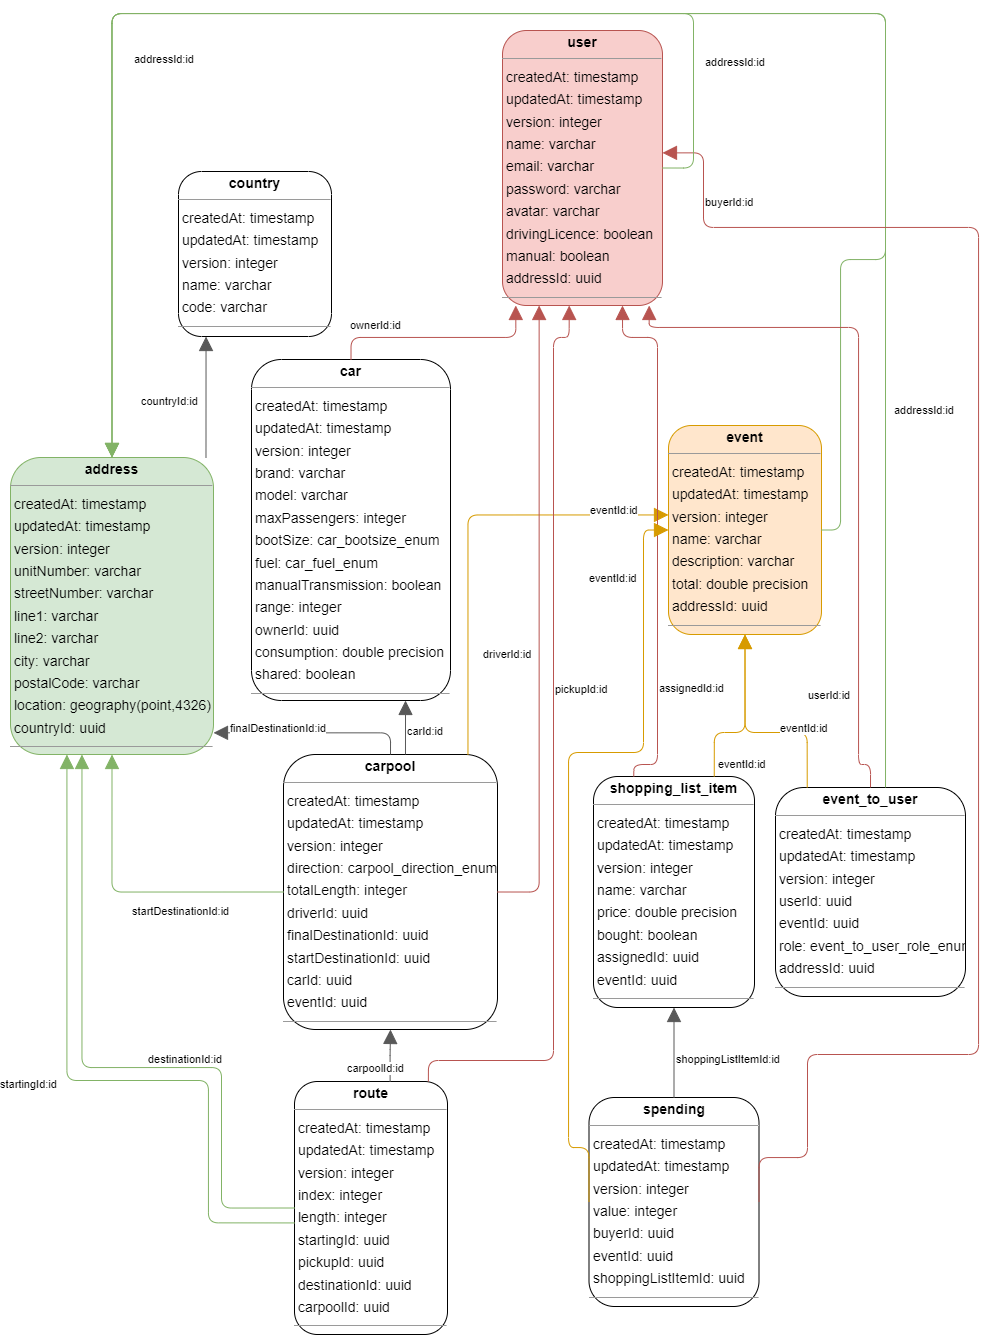
\includegraphics[width=\linewidth]{./images/dbShema}\caption{Architecture de la base de donnée}\label{fig:dbSchema}
    \centering
\end{figure}